\documentclass[aspectratio=169, 11pt]{beamer}

% ========== Theme ==========
\usetheme{Madrid}
\usecolortheme{whale}
\setbeamertemplate{navigation symbols}{}
\setbeamertemplate{footline}[frame number]

% ========== Packages ==========
\usepackage{tikz}
\usetikzlibrary{arrows.meta, positioning, shapes.geometric, calc, fit, backgrounds}
\usepackage{booktabs}
\usepackage{graphicx}
\usepackage{amsmath}
\usepackage{xcolor}

% ========== Colours ==========
\definecolor{highlight}{RGB}{220, 70, 70}
\definecolor{completed}{RGB}{80, 185, 100}
\definecolor{pending}{RGB}{180, 180, 180}
\definecolor{inprogress}{RGB}{90, 140, 240}

% ========== Title ==========
\title{Weekly Progress Report}
\subtitle{Week 31 --- Final Report Draft v10 Revision \& Template Alignment}
\author{Student ID: 11314389}
\institute{BCI Control System Project}
\date{April 21, 2026}

\begin{document}

% ===================================================
% TITLE PAGE
% ===================================================
\begin{frame}
    \titlepage
\end{frame}

% ===================================================
% SLIDE 1: Agenda
% ===================================================
\begin{frame}[shrink=8]{Week 31 Agenda --- Final Report Consolidation}

    \begin{block}{This Week's Main Work}
        \begin{enumerate}
            \item Rewrite the \textbf{Methodology} chapter based on the annotated feedback on the draft report.
            \item Check the report against the \textbf{3YP Handbook} and the official \textbf{Report Template}.
            \item Move the draft from a content-focused revision to a more submission-ready structure:
            \begin{itemize}
                \item front matter,
                \item chapter order,
                \item appendices,
                \item GitHub/repository evidence.
            \end{itemize}
            \item Resolve the final issues identified during re-review:
            \begin{itemize}
                \item Project Management location,
                \item over-strong claims in Discussion,
                \item Figure 1 readability,
                \item risk-assessment appendix references.
            \end{itemize}
        \end{enumerate}
    \end{block}

    \vspace{2mm}
    \begin{alertblock}{Outcome}
        Final Report Draft v10 has now been generated, restructured, and recompiled. The current PDF is 31 pages and is much closer to the handbook/template expectations than the previous draft.
    \end{alertblock}
\end{frame}

% ===================================================
% SLIDE 2: Methodology Rewrite
% ===================================================
\begin{frame}[shrink=7]{1. Methodology Revision Based on Feedback}

    \begin{columns}[T]
        \column{0.5\textwidth}
        \textbf{Main Problems in the Previous Draft}
        \begin{itemize}
            \item Methods and results were mixed together.
            \item Reproducibility details were incomplete.
            \item Some claims were too strong relative to the evidence.
            \item Dataset, preprocessing, and training protocol boundaries were unclear.
        \end{itemize}

        \vspace{1mm}
        \begin{exampleblock}{Core Revision Goal}
            The chapter should read as a \textbf{reproducible Methods chapter}, not as ``methods + partial results + interpretation''.
        \end{exampleblock}

        \column{0.48\textwidth}
        \textbf{Changes Implemented in v10}
        \begin{itemize}
            \item Results removed from Chapter 3 and concentrated in Chapter 4.
            \item Dataset table expanded with channels, sampling rates, class counts, and protocol.
            \item Preprocessing now specifies 8--30\,Hz filtering, epoching, and normalisation.
            \item EEGTransformer section now includes architecture figure, configuration table, and implementation details.
            \item Training strategy now states subject-dependent, LOSO, pooled pre-training, and fine-tuning protocols explicitly.
            \item RL section now defines state, action, reward, and network settings clearly.
        \end{itemize}
    \end{columns}
\end{frame}

% ===================================================
% SLIDE 3: Handbook / Template Alignment
% ===================================================
\begin{frame}[shrink=5]{2. Handbook and Template Alignment --- Structural Rework}

    \begin{columns}[T]
        \column{0.48\textwidth}
        \textbf{Handbook / Template Requirements Checked}
        \begin{itemize}
            \item A4, 2\,cm margins, 1.5 spacing, left-aligned text
            \item Calibri 12 or close equivalent
            \item Template-like front matter
            \item Main-body Project Management section
            \item Required appendices and GitHub link
        \end{itemize}

        \vspace{2mm}
        \begin{alertblock}{Font Constraint}
            True Calibri is not installed on this machine. The report now uses \textbf{XeLaTeX} with automatic fallback to \textbf{Carlito}, which is a close Calibri-compatible alternative.
        \end{alertblock}

        \column{0.5\textwidth}
        \textbf{Structural Changes Made}
        \begin{itemize}
            \item Added title page, abstract, declaration of originality, intellectual property statement, and acknowledgements.
            \item Renamed \textbf{Methodology} to \textbf{Methods} to match the template style.
            \item Added chapter-level introduction/summary structure in Literature Review, Methods, and Results \& Discussion.
            \item Restored \textbf{Project Management} to the main body.
            \item Added appendix sections for proposal, Gantt chart, risk material, CPD log, and repository link.
        \end{itemize}
    \end{columns}
\end{frame}

% ===================================================
% SLIDE 4: Remaining Issues Fixed
% ===================================================
\begin{frame}[shrink=8]{3. Final Review Fixes Completed This Week}

    \begin{table}
        \centering
        \small
        \begin{tabular}{p{4.0cm}p{6.0cm}c}
            \toprule
            \textbf{Issue} & \textbf{Action Taken} & \textbf{Status} \\
            \midrule
            Project Management not in main body
            & Added a dedicated main-body chapter before Conclusions
            & \textcolor{completed}{Fixed} \\
            Discussion claims too strong
            & Reworded several interpretive claims using more cautious evidence-based language
            & \textcolor{completed}{Fixed} \\
            Figure 1 text too small
            & Removed hard full-width shrink, enlarged internal font, tightened layout
            & \textcolor{completed}{Fixed} \\
            Risk appendix path outdated
            & Updated appendix reference to the new files in \texttt{05\_Documentation}
            & \textcolor{completed}{Fixed} \\
            Overuse of ``subject''
            & Partially normalised to ``participant'' in the revised sections
            & \textcolor{inprogress}{Improved} \\
            \bottomrule
        \end{tabular}
    \end{table}

    \vspace{2mm}
    \begin{exampleblock}{New Risk Files Referenced}
        \texttt{05\_Documentation/Risk assessment form-11314389\_v3.docx}\\
        \texttt{05\_Documentation/Risk assessment form-11314389\_v3.pdf}
    \end{exampleblock}
\end{frame}

% ===================================================
% SLIDE 5: Current Draft Status
% ===================================================
\begin{frame}[shrink=9]{4. Current Draft v10 --- Report Status Summary}

    \begin{table}
        \centering
        \small
        \begin{tabular}{llc}
            \toprule
            \textbf{Area} & \textbf{Current v10 Status} & \textbf{State} \\
            \midrule
            Methodology chapter          & Rewritten around reproducibility and protocol clarity & \textcolor{completed}{\checkmark} \\
            Results chapter separation   & Quantitative outcomes moved out of Methods            & \textcolor{completed}{\checkmark} \\
            EEGTransformer documentation & Figure + config table + implementation detail         & \textcolor{completed}{\checkmark} \\
            RL formulation               & State/action/reward/network protocol specified        & \textcolor{completed}{\checkmark} \\
            Front matter                 & Template-style title and declaration pages added      & \textcolor{completed}{\checkmark} \\
            Project Management           & Back in main body                                     & \textcolor{completed}{\checkmark} \\
            Appendices                   & Structure added; risk files now concretely referenced & \textcolor{completed}{\checkmark} \\
            PDF compilation              & XeLaTeX build successful                              & \textcolor{completed}{\checkmark} \\
            Font                         & Carlito fallback, not true Calibri                    & \textcolor{pending}{Known limit} \\
            Missing appendix artefacts   & Proposal / Gantt / CPD still need final inserted copies & \textcolor{pending}{Needs final package} \\
            \bottomrule
        \end{tabular}
    \end{table}

    \vspace{2mm}
    \begin{center}
        \textbf{Current compiled report length: 31 pages}
    \end{center}
\end{frame}

% ===================================================
% SLIDE 6: What Changed in the Report Itself
% ===================================================
\begin{frame}[shrink=5]{5. What the Marker Now Sees in v10}

    \begin{columns}[T]
        \column{0.5\textwidth}
        \textbf{Front of Report}
        \begin{itemize}
            \item Title page and front matter completed
            \item Abstract with key numerical results
            \item Declaration of originality
            \item Intellectual property statement
            \item Acknowledgements
        \end{itemize}

        \vspace{2mm}
        \textbf{Middle of Report}
        \begin{itemize}
            \item Methods rewritten to read like a proper protocol chapter
            \item Results and Discussion separated cleanly
            \item Project Management included in the main body
        \end{itemize}

        \column{0.48\textwidth}
        \textbf{End of Report}
        \begin{itemize}
            \item Conclusions and Future Work
            \item References
            \item Appendix placeholders converted into structured appendix sections
            \item GitHub repository link included
            \item Risk-assessment files now explicitly referenced
        \end{itemize}

        \vspace{2mm}
        \begin{alertblock}{Most Important Improvement}
            The draft now looks much more like a final-year report submission and much less like a technical write-up assembled section by section.
        \end{alertblock}
    \end{columns}
\end{frame}

% ===================================================
% SLIDE 7: Timeline and Next Steps
% ===================================================
\begin{frame}{6. Timeline and Next Steps}

    \begin{center}
    \scalebox{0.8}{%
    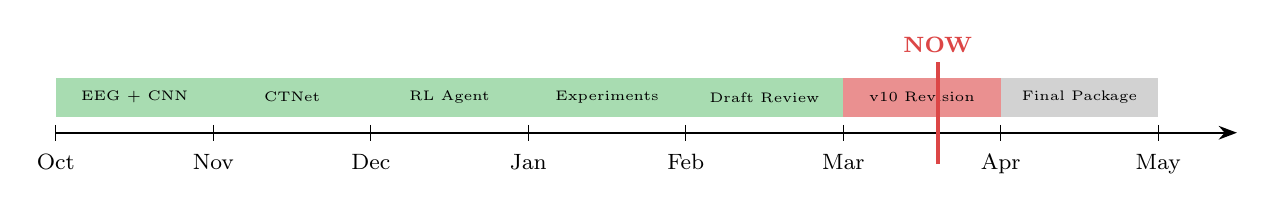
\begin{tikzpicture}
        \draw[thick, -Stealth] (0,0) -- (15,0);
        \foreach \x/\m in {0/Oct, 2/Nov, 4/Dec, 6/Jan, 8/Feb, 10/Mar, 12/Apr, 14/May} {
            \draw (\x, 0.1) -- (\x, -0.1);
            \node[below, font=\footnotesize] at (\x, -0.15) {\m};
        }
        \fill[completed!50]  (0,  0.2) rectangle (2,  0.7); \node[font=\tiny] at (1,   0.45) {EEG + CNN};
        \fill[completed!50]  (2,  0.2) rectangle (4,  0.7); \node[font=\tiny] at (3,   0.45) {CTNet};
        \fill[completed!50]  (4,  0.2) rectangle (6,  0.7); \node[font=\tiny] at (5,   0.45) {RL Agent};
        \fill[completed!50]  (6,  0.2) rectangle (8,  0.7); \node[font=\tiny] at (7,   0.45) {Experiments};
        \fill[completed!50]  (8,  0.2) rectangle (10, 0.7); \node[font=\tiny] at (9,   0.45) {Draft Review};
        \fill[highlight!60]  (10, 0.2) rectangle (12, 0.7); \node[font=\tiny] at (11,  0.45) {v10 Revision};
        \fill[pending!60]    (12, 0.2) rectangle (14, 0.7); \node[font=\tiny] at (13,  0.45) {Final Package};

        \draw[highlight, ultra thick] (11.2, -0.4) -- (11.2, 0.9);
        \node[highlight, above, font=\footnotesize\bfseries] at (11.2, 0.9) {NOW};
    \end{tikzpicture}}
    \end{center}

    \vspace{1mm}
    \begin{exampleblock}{Completed This Week}
        \textbf{1.} Methodology rewritten based on feedback \quad
        \textbf{2.} Handbook/template alignment completed \quad
        \textbf{3.} Final review issues resolved \quad
        \textbf{4.} v10 compiled and verified
    \end{exampleblock}

    \begin{block}{Next Steps Before Submission}
        \small
        \begin{itemize}
            \item Insert the final copies of the proposal, Gantt chart, and CPD artefacts into the appendix package.
            \item Perform one last language-and-consistency pass across the full report.
            \item Confirm that the current 31-page main body stays within the handbook page limit after final appendix packaging.
        \end{itemize}
    \end{block}
\end{frame}

\end{document}
